\documentclass{article}
\usepackage{styles/report}
\usepackage{styles/codespace}

%%%%% Variables %%%%%%
%\setprojectname{}
%\setreportname{}
%\setreportcode{fill this in}
%\setaxilleasrole{fill this in}
%\setbillrole{fill this in}
\setplatrole{Σύνταξη τεχνικού κειμένου (v0.1)}
\sethalvasrole{Σύνταξη τεχνικού κειμένου (v0.2, v1.0)}

%\addtolength{\cftsecnumwidth}{52pt}
\renewcommand\thesection{\arabic{section}:}
\renewcommand\thesubsection{\arabic{section}.\alph{subsection}}
\renewcommand\thesubsubsection{\arabic{section}.\alph{subsection}.\roman{subsubsection}}

\reportlayout
\begin{document}
\coverpages

\section{Διάγραμμα Gantt}
\begin{figure}[!htb]
  \centering
    \centering
    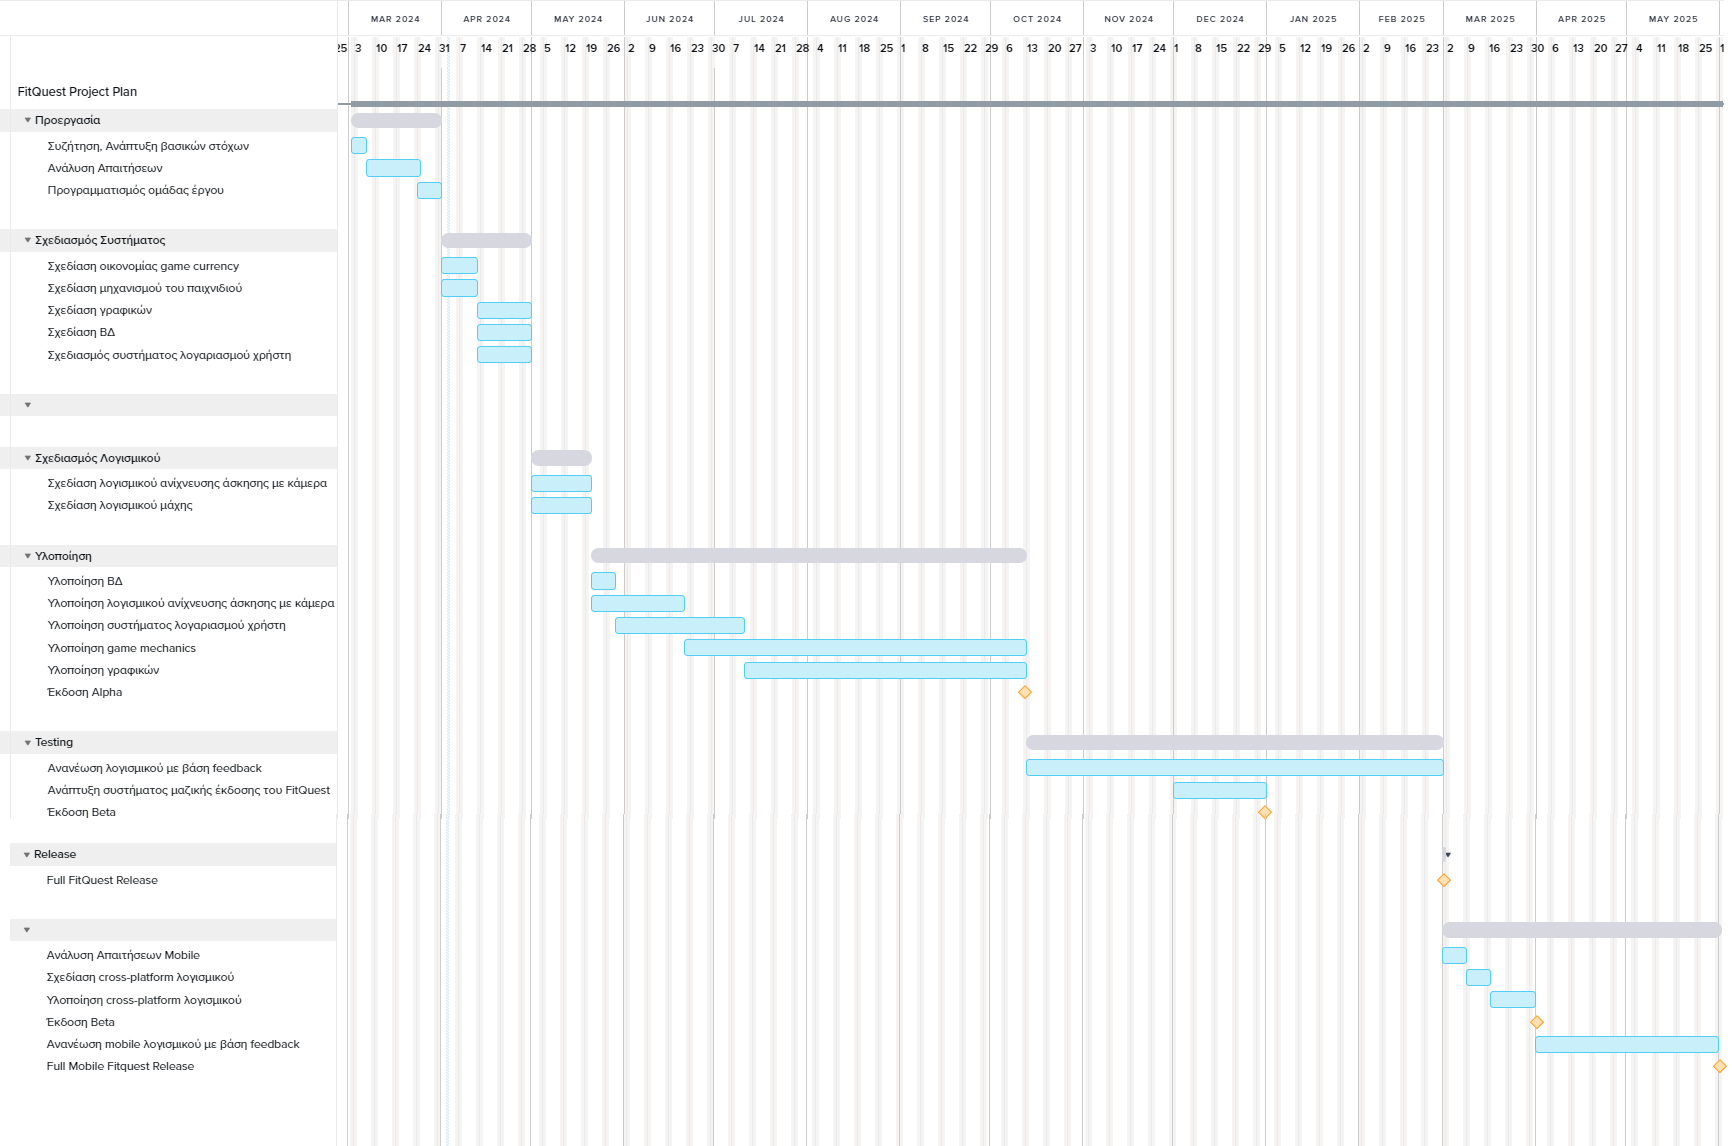
\includegraphics[width=18Cm,height=20cm]{project-gant-updates.jpg}
    \caption{Gantt Chart}
    \label{}
\end{figure}
\begin{flushleft}
Η πραγματοποίηση της παραγωγής της mobile έκδοσης (3 τελευταίοι μήνες του project plan) θα εξαρτηθεί από την τελική διάρκεια της παραγωγής της αρχικής desktop έκδοσης και του feedback που θα πάρει η ομάδα μας από την beta έκδοση.
\end{flushleft}
\section{Mockups}
\textbf{ Για τη δημιουργία των Mockups χρησιμοποιήθηκε το λογισμικό adobe photoshop }

\begin{figure}[!htb]
  \centering
    \centering
    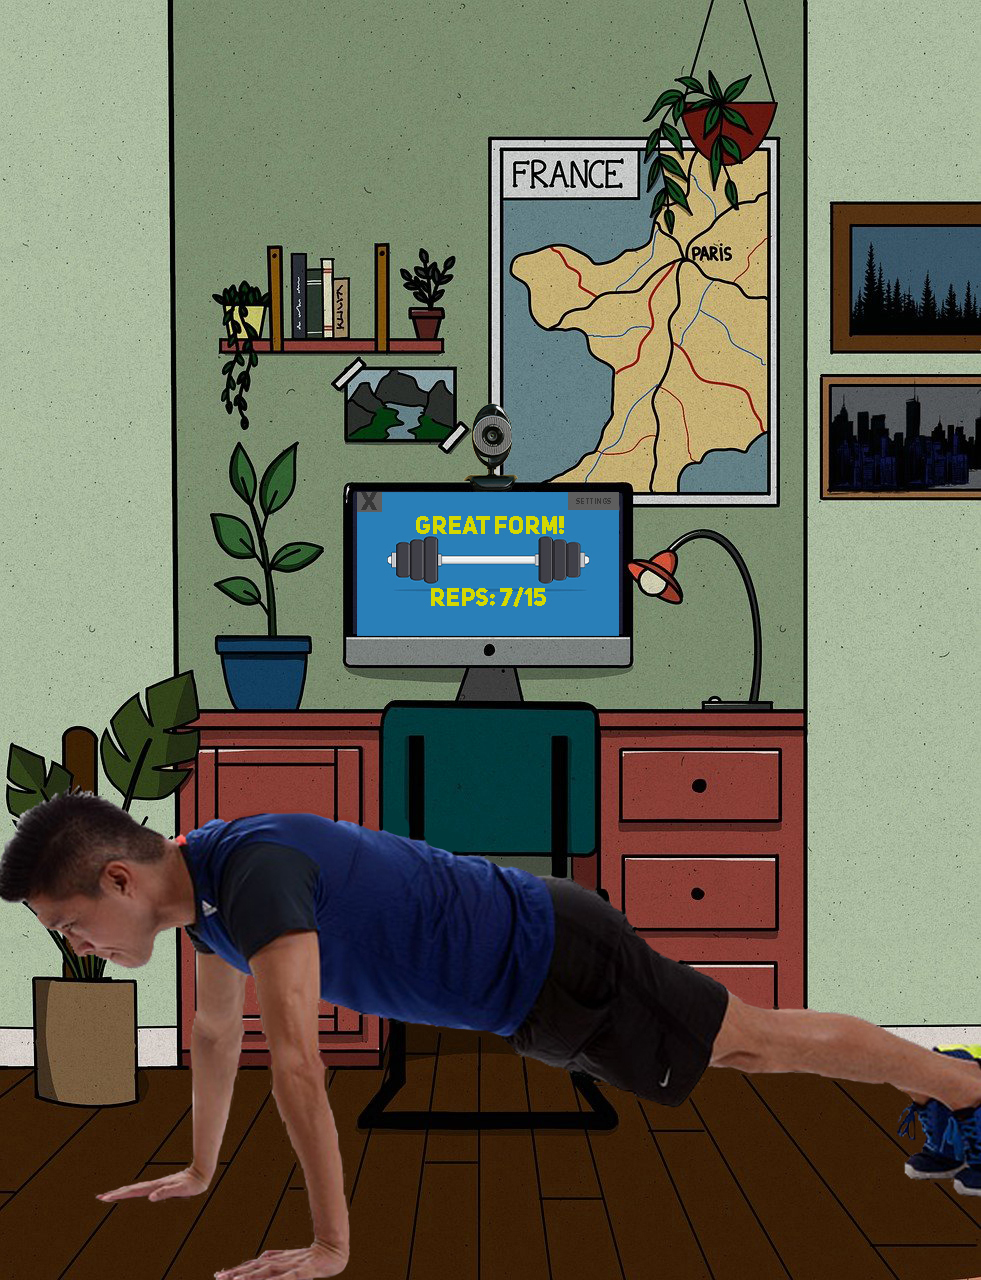
\includegraphics[width=\textwidth]{mockup1.jpg}
    \caption{Camera preview}
    \label{}
\end{figure}


\begin{figure}[h]
    \centering
    \begin{minipage}[b]{0.45\textwidth}
        \centering
    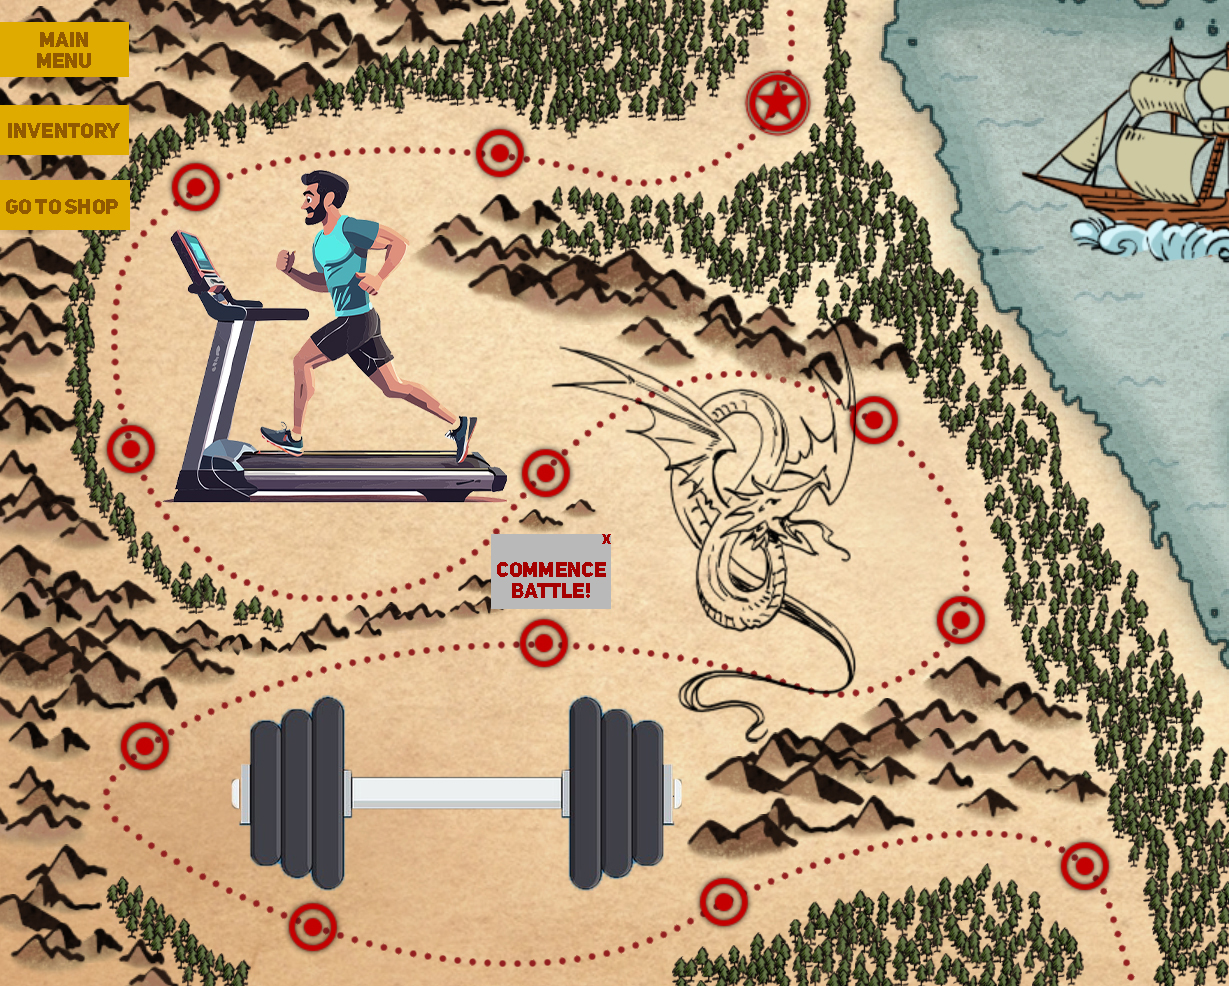
\includegraphics[width=\textwidth]{omockup2.jpg}
    \caption{Mockup': Map preview}
    \end{minipage}
    \hfill
    \begin{minipage}[b]{0.45\textwidth}
        \centering
    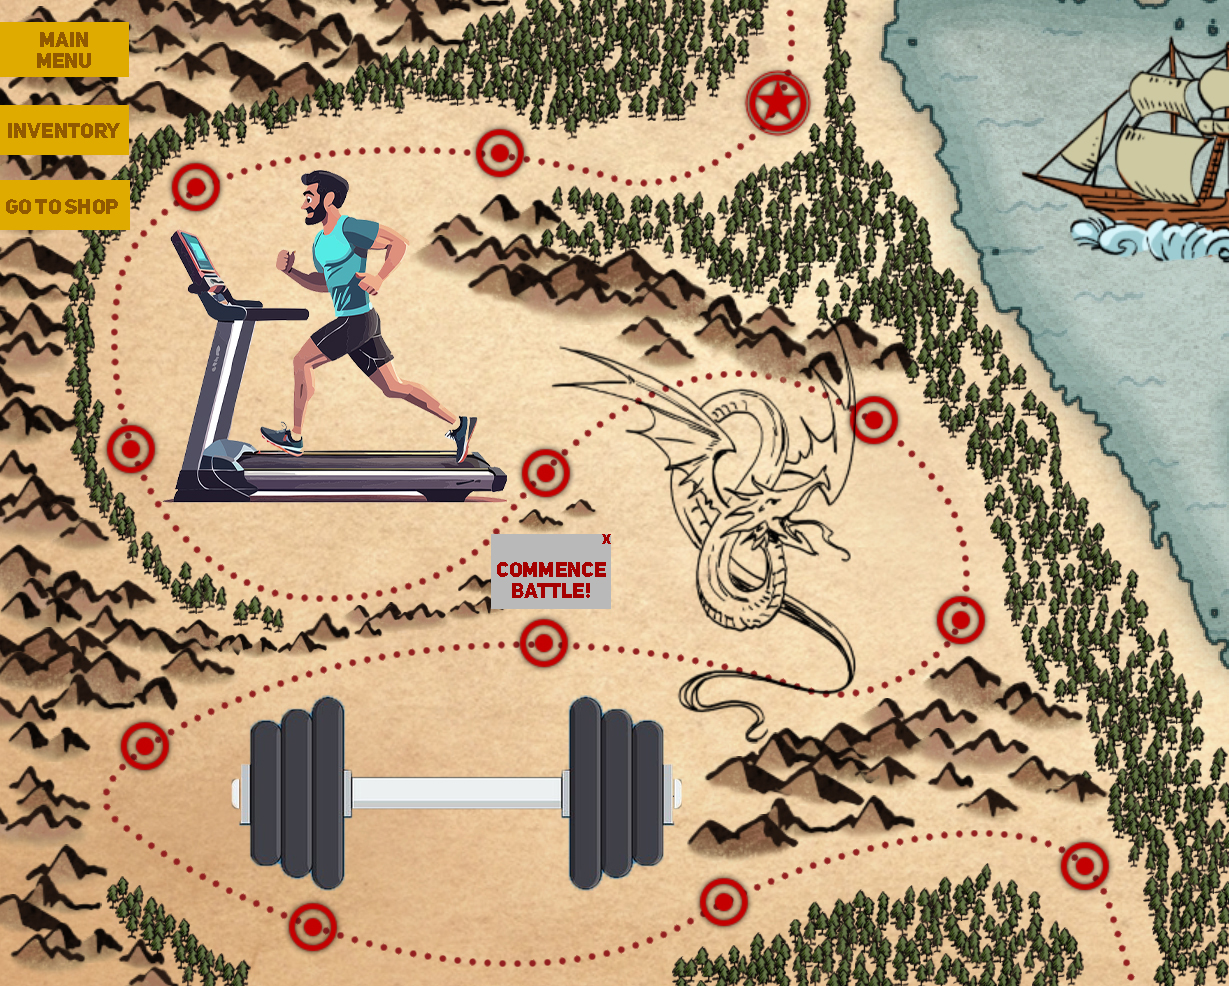
\includegraphics[width=\textwidth]{mockup2.jpg}
    \caption{Map preview}
    \end{minipage}
\end{figure}


\begin{figure}[h]
    \centering
    \begin{minipage}[b]{0.45\textwidth}
        \centering
    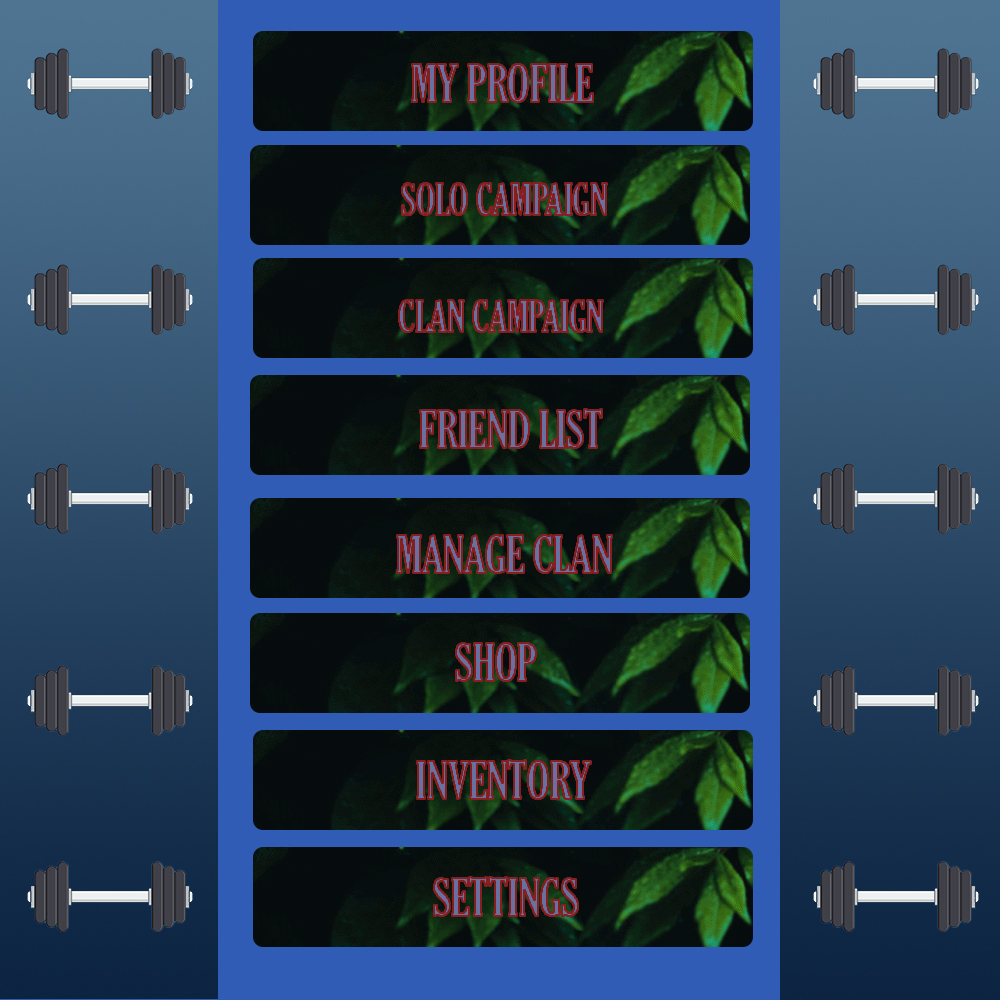
\includegraphics[width=\textwidth]{omockup3.jpg}
    \caption{Mockup: Main menu}
    \end{minipage}
    \hfill
    \begin{minipage}[b]{0.45\textwidth}
        \centering
    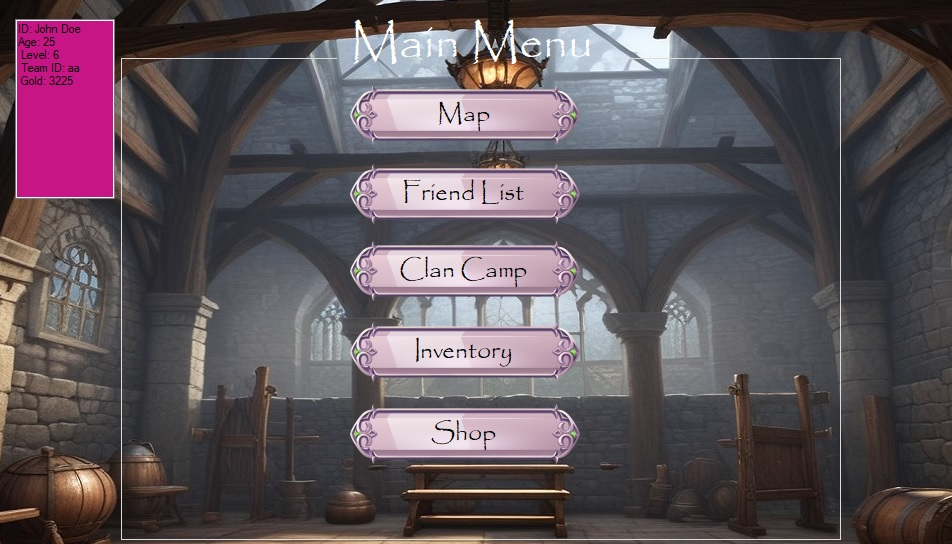
\includegraphics[width=\textwidth]{mockup3.jpg}
    \caption{Main menu}
    \end{minipage}
\end{figure}



\begin{figure}[h]
    \centering
    \begin{minipage}[b]{0.45\textwidth}
        \centering
    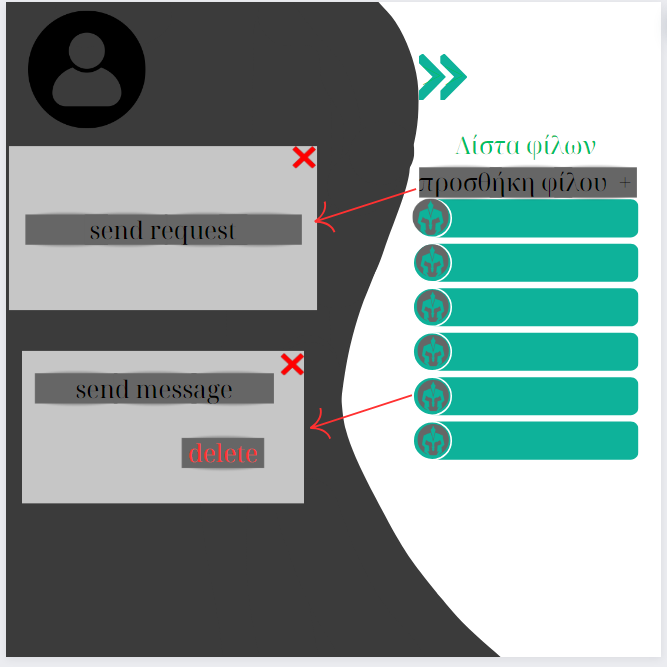
\includegraphics[width=\textwidth]{omockup4.jpg}
    \caption{Mockup: Friends list}
    \end{minipage}
    \hfill
    \begin{minipage}[b]{0.45\textwidth}
        \centering
    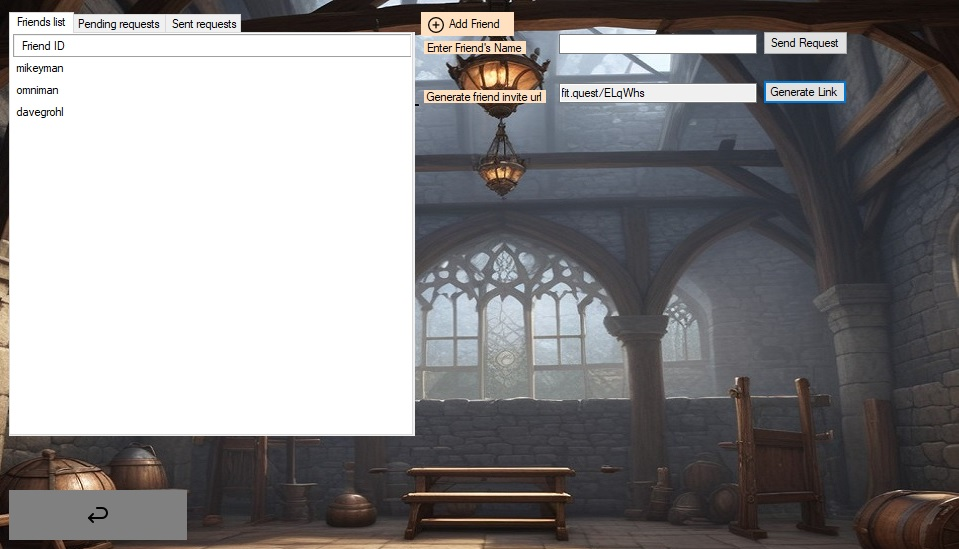
\includegraphics[width=\textwidth]{mockup4.jpg}
    \caption{Friends list}
    \end{minipage}
\end{figure}

\begin{figure}[h]
    \centering
    \begin{minipage}[b]{0.45\textwidth}
        \centering
    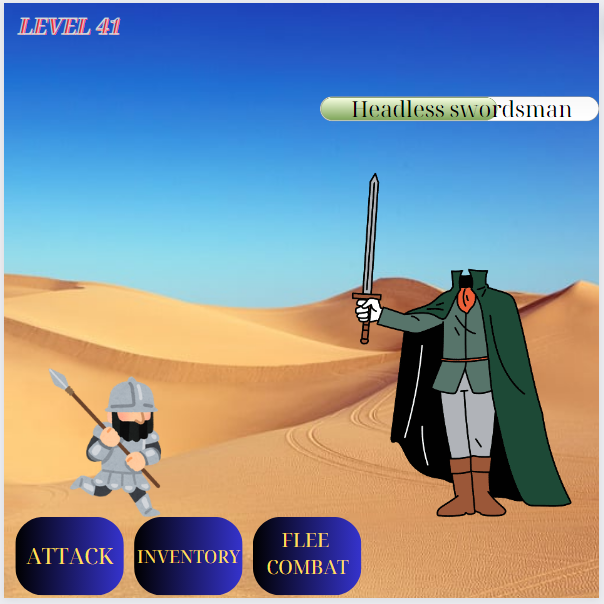
\includegraphics[width=\textwidth]{omockup5.jpg}
    \caption{Mockup: Solo combat}
    \end{minipage}
    \hfill
    \begin{minipage}[b]{0.45\textwidth}
        \centering
    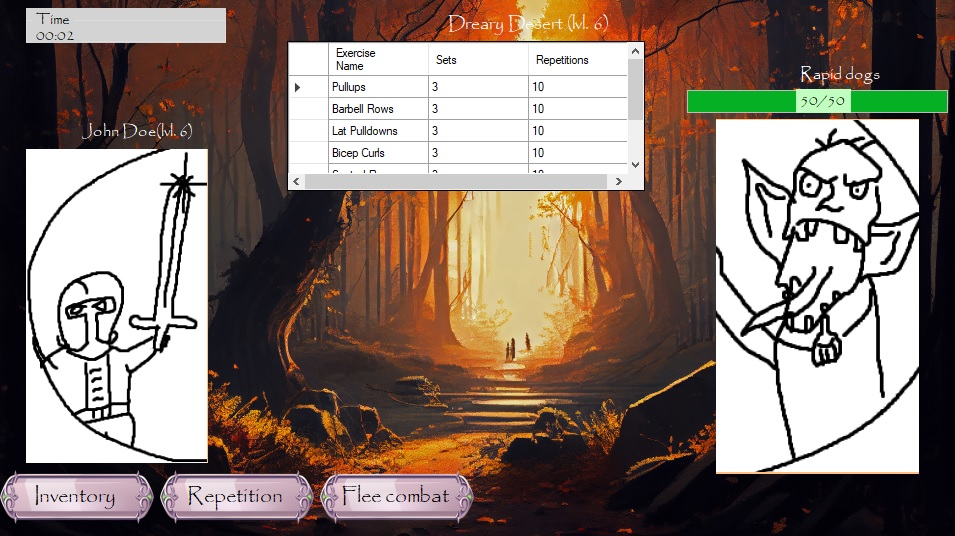
\includegraphics[width=\textwidth]{mockup5.jpg}
    \caption{Solo combat}
    \end{minipage}
\end{figure}




\begin{figure}[h]
    \centering
    \begin{minipage}[b]{0.45\textwidth}
        \centering
    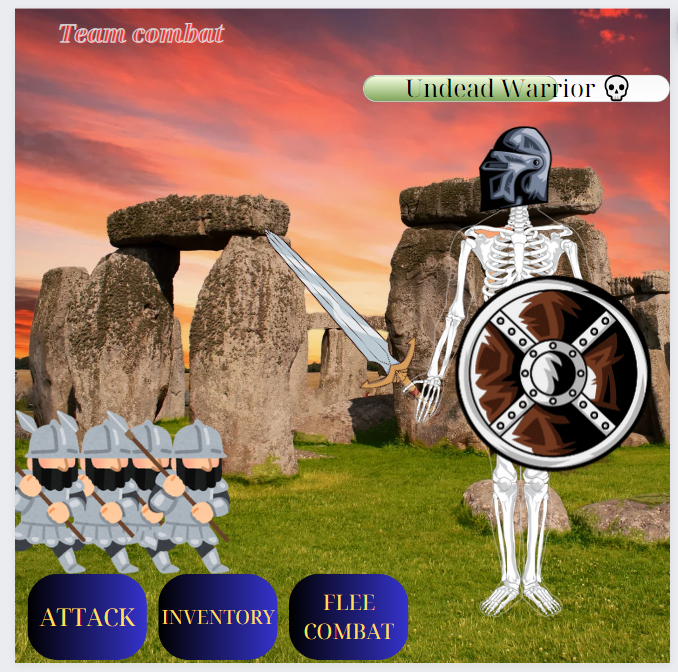
\includegraphics[width=\textwidth]{omockup6.jpg}
    \caption{Mockup: Clan combat}
    \end{minipage}
        \hfill
    \begin{minipage}[b]{0.45\textwidth}
        \centering
    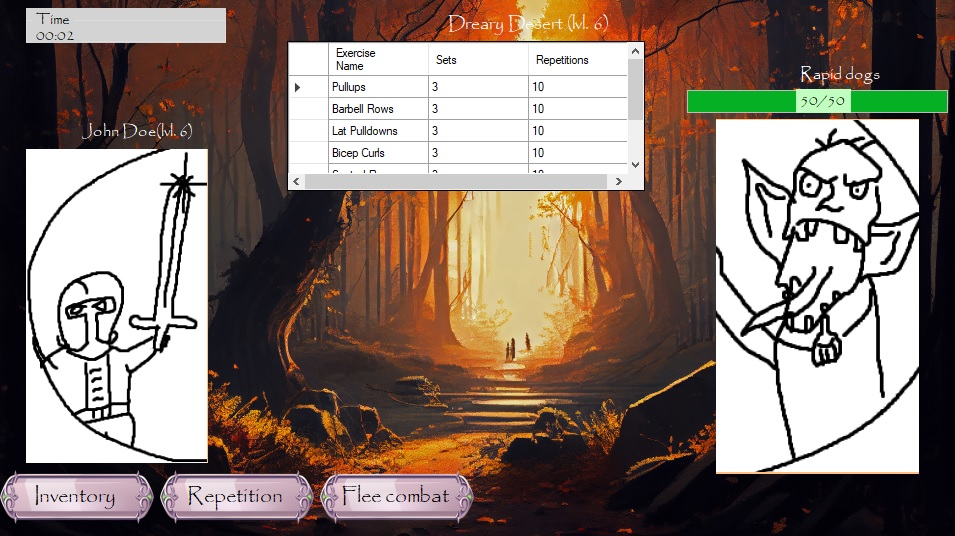
\includegraphics[width=\textwidth]{mockup5.jpg}
    \caption{Clan combat}
    \end{minipage}
\end{figure}



\begin{figure}[h]
    \centering
    \begin{minipage}[b]{0.45\textwidth}
        \centering
    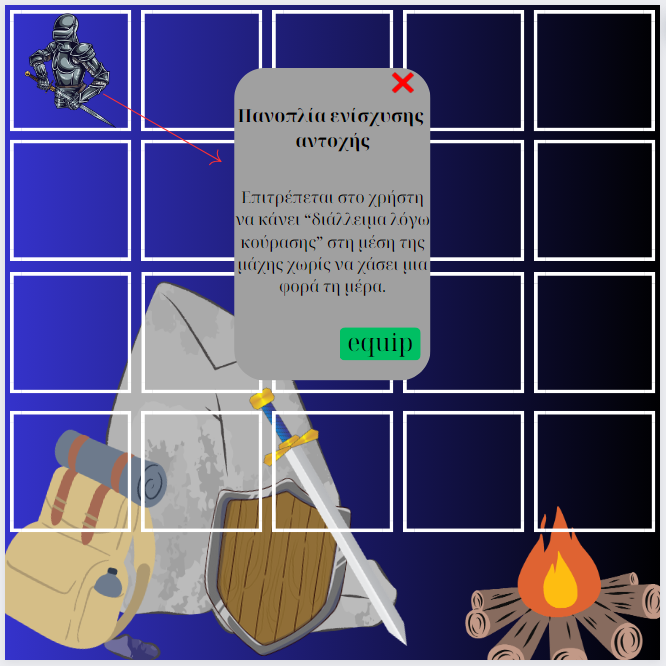
\includegraphics[width=\textwidth]{omockup7.jpg}
    \caption{Mockup: Inventory}
    \end{minipage}
    \hfill
    \begin{minipage}[b]{0.45\textwidth}
        \centering
    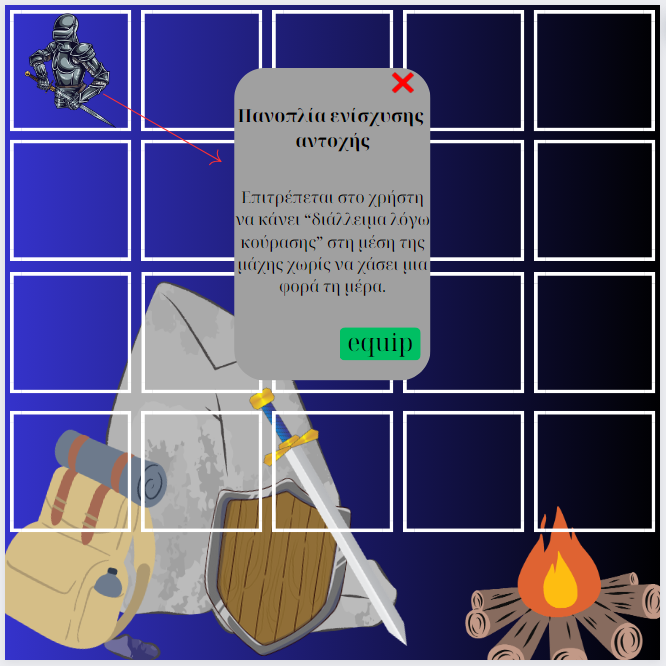
\includegraphics[width=\textwidth]{mockup7.jpg}
    \caption{Inventory}
    \end{minipage}
\end{figure}



\begin{figure}[h]
    \centering
    \begin{minipage}[b]{0.45\textwidth}
        \centering
    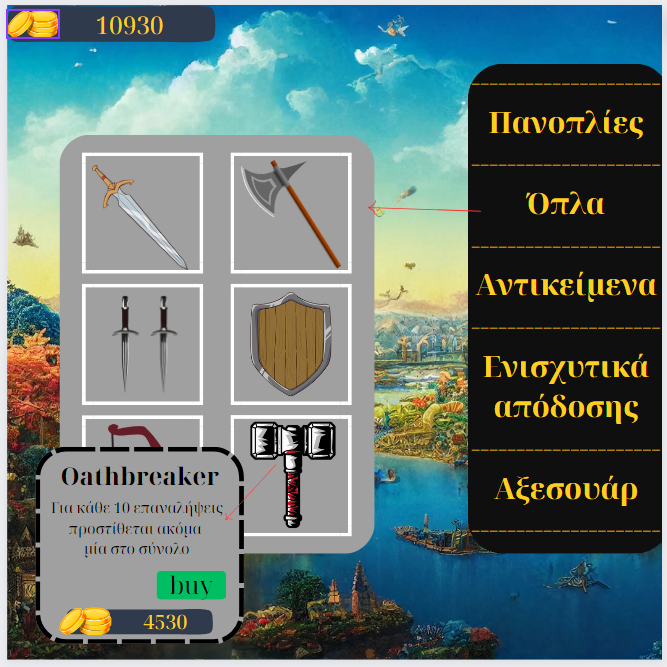
\includegraphics[width=\textwidth]{omockup8.jpg}
    \caption{Mockup: {Shop}}
    \end{minipage}
    \hfill
    \begin{minipage}[b]{0.45\textwidth}
        \centering
    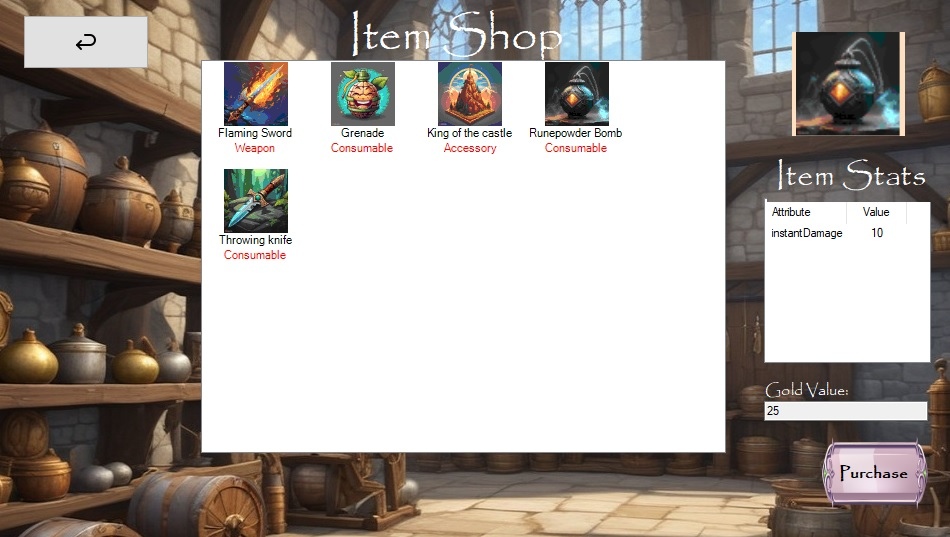
\includegraphics[width=\textwidth]{mockup8.jpg}
    \caption{Shop}
    \end{minipage}
\end{figure}


	
\begin{figure}[!htb]
  \centering
    \centering
    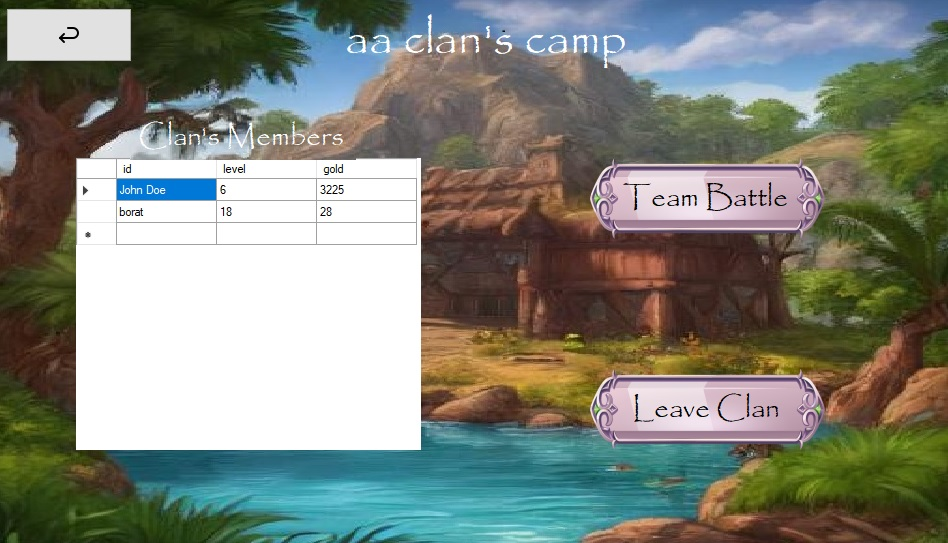
\includegraphics[width=\textwidth]{mockup9.jpg}
    \caption{Clan camp}
    \label{}
\end{figure}


\bibliographystyle{plain}
\renewcommand*\refname{Βιβλιογραφία}
\bibliography{refs}
Όλα τα τα στοιχεία που χρησιμοποιήθηκαν στις μακέτες βρίσκονται στο https://pixabay.com/ \newline και στο https://www.canva.com/
\end{document}
